% 9 variables in here:
% h_1 = 10.0, h_2 = 10.0, h_3 = 10.0, ux_1 = 0.0, ux_2 = 0.0, ux_3 = 0.0, uy_1 = 0.0, uy_2 = 0.0, uy_3 = 0.0
\begin{figure}[h!]
\centering
  \subfigure[1st basis function, $x$-momentum] {
    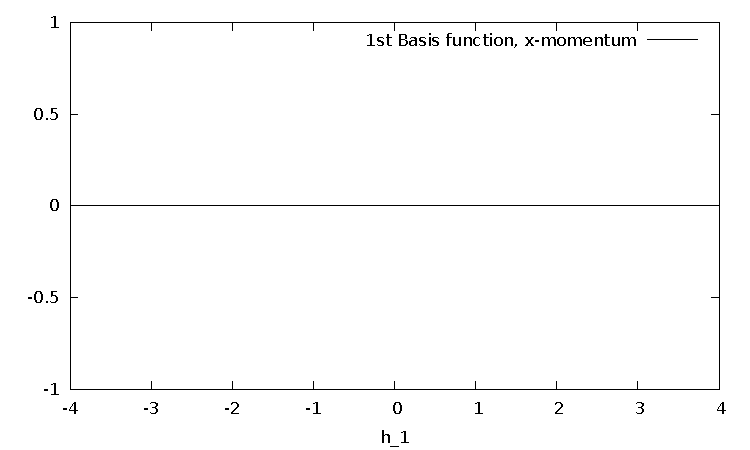
\includegraphics[scale=\zoomfactor]{{{standardwerte_nach_h1_ord1/y_10.0_10.0_0.0_0.0_0.0_0.0_0.0_0.0f0}}}
  }
  \subfigure[1st basis function, $y$-momentum] {
    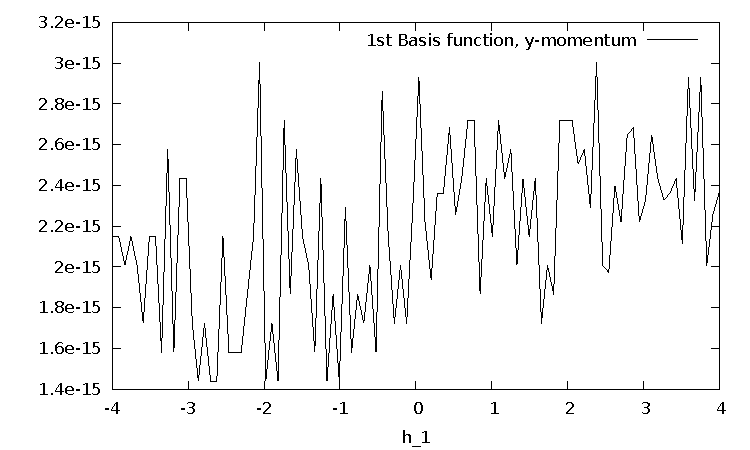
\includegraphics[scale=\zoomfactor]{{{standardwerte_nach_h1_ord1/y_10.0_10.0_0.0_0.0_0.0_0.0_0.0_0.0f1}}}
  }
  \subfigure[2nd basis function, $x$-momentum] {
    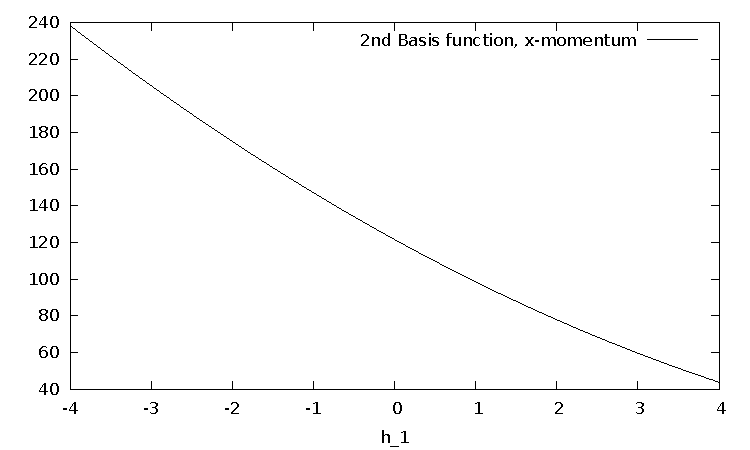
\includegraphics[scale=\zoomfactor]{{{standardwerte_nach_h1_ord1/y_10.0_10.0_0.0_0.0_0.0_0.0_0.0_0.0f2}}}
  }
  \subfigure[2nd basis function, $y$-momentum] {
    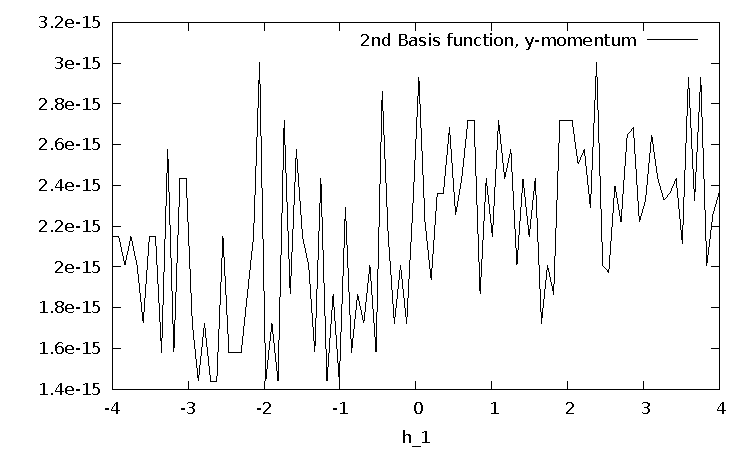
\includegraphics[scale=\zoomfactor]{{{standardwerte_nach_h1_ord1/y_10.0_10.0_0.0_0.0_0.0_0.0_0.0_0.0f3}}}
  }
  \subfigure[3rd basis function, $x$-momentum] {
    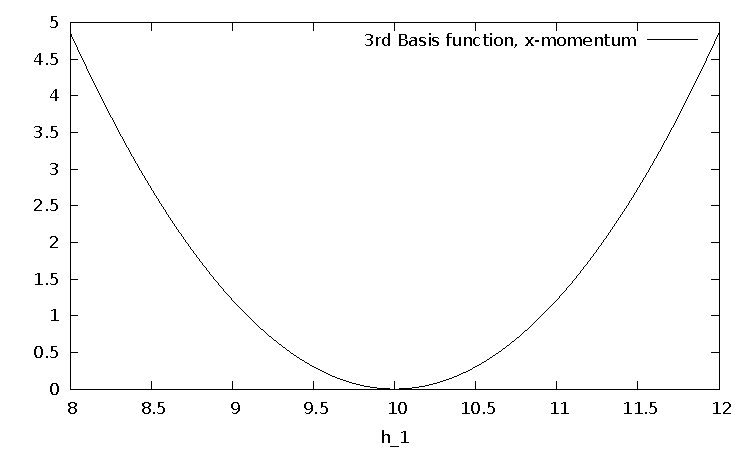
\includegraphics[scale=\zoomfactor]{{{standardwerte_nach_h1_ord1/y_10.0_10.0_0.0_0.0_0.0_0.0_0.0_0.0f4}}}
  }
  \subfigure[3rd basis function, $y$-momentum] {
    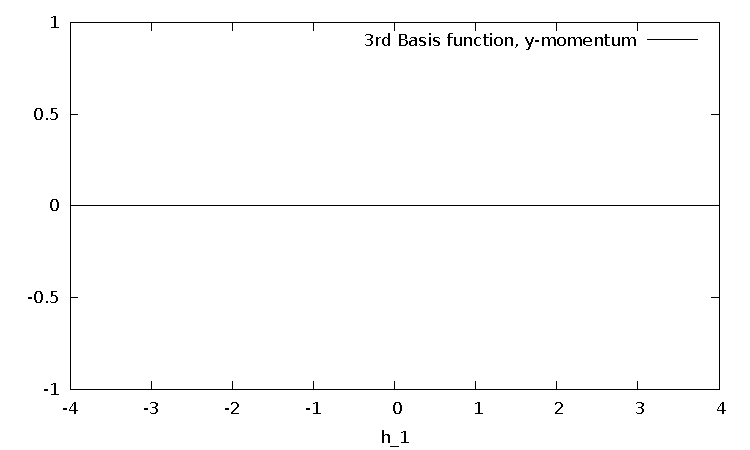
\includegraphics[scale=\zoomfactor]{{{standardwerte_nach_h1_ord1/y_10.0_10.0_0.0_0.0_0.0_0.0_0.0_0.0f5}}}
  }
\caption{Error plots for order 1. Values of variables are 
  $h_2 = 10 , h_3 = 10,
  u_{x,1} = 0 , u_{x,2} = 0 , u_{x,3} = 0 ,
  u_{y,1} = 0 , u_{y,2} = 0 , u_{y,3} = 0$. $h_1$ is varying.}
\label{fig:stiffness-analysis-order-1-standard-values-h1}
\end{figure}
